\documentclass[journal, a4paper]{IEEEtran}

\usepackage{cite}
\usepackage{amsmath}
\usepackage{amssymb}
\usepackage{graphicx}
\usepackage{url}
\usepackage[usenames, dvipsnames]{color}

\begin{document}

\title{Scaling of Electrode-Electrolyte Interface Model Parameters In Phosphate Buffered Saline}

\author{Mark~H.~Jones and Jonathan~Scott,~\IEEEmembership{Senior Member,~IEEE}
\thanks{Mark~H.~Jones is with the School of Electronic Engineering, University of Waikato, New Zealand, e-mail: markjones112358@gmail.com.}%
\thanks{Jonathan Scott is with the School of Electronic Engineering, University of Waikato, New Zealand.}
}

\markboth{Transactions on Biomedical Circuits and Systems}
{Jones \MakeLowercase{\textit{et al.}}: Scaling of Electrode-Electrolyte Interface Model Parameters in Phosphate Buffered Saline\...}
\maketitle



\begin{abstract}

We report how the impedance presented by a platinum electrode scales with the concentration of phosphate buffered saline (PBS).
We find that the constant phase element of the model scales with approximately the log of concentration, whereas the resistivity is inversely proportional.
Using a novel DC measurement technique we show that the Faradaic response of a platinum electrode, and thus the safe exposure limit, does not scale with concentration below 900\thinspace mV overpotential across a pair of electrodes.
We compare objective measurements made in saline to those made in the spinal cavity of live sheep. We comment upon the appropriateness of using PBS as a substitute for in-vivo measurements.
\end{abstract}

\begin{IEEEkeywords}
    Electrical stimulation, Bioelectric phenomena, Biophysics, Bioimpedance, Biomedical electrodes, Biomedical measurements, Implantable biomedical devices
\end{IEEEkeywords}




\section{Introduction}

\IEEEPARstart{T}{here} is considerable interest in the electrical modelling of electrodes. \cite{Cogan2008,Troy2006}
In \cite{Franks2005} a linearised model was presented, and in \cite{ScottSingle2013} a non-linear model
suitable for use with the SPICE circuit simulator was presented. The SPICE model usefully characterises an electrode in a given electrolyte with a small number of parameters.
One major reason for the interest in the electrical impedance of electrodes concerns the design of electronics intended for integration into pacemakers, cochlear implants, spinal cord stimulators, etc. The design of successful circuits depends upon a good understanding of external load impedance, while maximisation of battery life is linked to the use of electrodes whose impedance is well understood.
Having a compact model of an electrode in the appropriate electrolyte allows circuit designers to simulate their designs with valid loads. Knowing the effect upon the model of changes in the electrode or electrolyte would allow designers to anticipate circumstances that will affect the load seen by their circuits. Another appeal of a compact model stems from the fact that electrode characteristics are succinctly and objectively represented by the model parameters. These enable direct comparison of different electrodes, or the change in electrode properties over time. For example, in \cite{Kane13} changes in chronically-implanted electrodes are observed but there is no standard quantitative way of presenting the changes. Similarly, while there is a good understanding of what represents safe exposure, a compact model with parameters permits the prediction of the safety of any given stimulus regime.~\cite{Merrill05}

Electrodes in the laboratory are typically tested in a saline solution selected to mimic the circumstances in which they will operate when implanted.
In an implanted setting there is no reference electrode and many of the well established electrochemical measurement regimes do not apply. In this manuscript we measure the behaviour an electrode/electrolyte situation as it would be seen from an implant device.

A solution of Phosphate Buffered Saline (PBS) diluted to one-tenth concentration (0.1X) is common in the case of Spinal Cord Stimulators (SCS), while full concentration (1.0X) PBS is considered more representative of the situation in blood.

In this manuscript we report how the parameters of a non-linear model change as the concentration of saline is varied. We refine a series of measurements compatible with commercially available medical electrodes in physiological saline that allow us to describe the impedance with minimal parameters. We place these parameters in context with a biological measurement made in the spinal cavity of a live sheep.

The electrode used in this work is a commercial linear array of eight platinum electrodes intended for SCS implantation called an ``Octrode''.~\cite{StJudeOctrode} A picture of an Octrode is presented in figure~\ref{fig:octrode}.
The electrical interface model of \cite{Franks2005} and \cite{ScottSingle2013} has two parts, a displacement branch and a Faradaic branch. While Scott and Single \cite{ScottSingle2013} incorporate a memristor into their model, it has been omitted here for simplicity. Its contribution is limited to situations where diffusion limited Faradaic reactions come into play, a situation that stimulator implants are designed to avoid.

It has been suggested that the primary coupling mechanism between platinum electrodes and physiological saline is the reversible evolution of gas, probably oxygen, at the platinum surface, which dissolves without bubble formation.\cite{Greatbatch1969} Understanding the exact mechanism of displacement or Faradaic charge transfer at the electrode surface is beyond the scope of this work. Rather we wish to characterise the electrode/electrolyte system in terms of parameters that may be fed into an electrical model.

\begin{figure}
    \begin{center}
    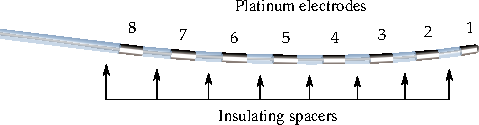
\includegraphics{graphics/StJudeOctrodeDiagram}
    \end{center}
    \caption{St. Jude Medical Octrode lead comprised of eight coaxial cylindrical platinum electrodes (1mm in diameter, 3mm long) separated by 4mm insulating spacers.}
    \label{fig:octrode}
\end{figure}

\begin{figure}
    \begin{center}
        
\includegraphics[width=230pt]{graphics/interfaceSchematic_noMemristive}
    \end{center}
    \caption{Electrical schematic of the electrode-interface impedance model used in this work. $D_{a}$ and $D_{b}$ represent diodes; $CPE$ and $R_{s}$ represent the constant phase element and series resistance respectively.}
    \label{fig:schematic}
\end{figure}

\section{Resistive Network}
Six solutions ranging from 1.0X to 0.025X the concentration of a stock PBS solution have been examined.
The ingredients of that stock solution are given in table~\ref{tab:PBSrecipe}.
The pH level of the stock was measured, using a calibrated EDT Instruments BA-350 pH meter, to have a pH of 7.4. No pH adjustments were made to the derived solutions.

\begin{table}
    \begin{center}
        \begin{tabular}{|r|l|}
            \hline
            $NaCl$ & $8.0\thinspace g$ \\ \hline
            $KCl$ & $0.2\thinspace g$ \\ \hline
            $Na_{2}HPO_{4}$ & $1.44\thinspace g$ \\ \hline
            $KH_{2}PO_{4}$ & $0.24\thinspace g$ \\ \hline
            Distilled Water & $1.0$\thinspace L \\ \hline
        \end{tabular}
    \end{center}
    \caption{PBS stock solution ingredients}
    \label{tab:PBSrecipe}
\end{table}

The electrical impedance between two electrodes in an electrolyte arises from two interface impedances in series with the resistance due to the bulk of the electrolyte itself. To quantify the impedance presented by a single interface we first need to understand the inter-electrode resistances presented by the electrolyte bulk. As there are always two interface impedances between any two electrodes, inter-electrode resistances cannot be measured in isolation.

In \cite{ScottSingle2013}, a series of transresistance measurements were used in conjunction with a physical description of the electrode geometry to build up a representative network of resistors. The network in that paper was defined using five parameters: $R_{eri}$, $R_{lri}$, $R_{li}$, mesh depth, and edge depth. Readers are referred to \cite{ScottSingle2013} for the interpretation of these model parameters. Repeating that work, a resistor network that connects each of the eight electrodes is constructed, mimicking the resistances due to the solution bulk.

The mesh depth and padding values of five columns and three rows, respectively, has been taken directly from \cite{ScottSingle2013}.
A numerical fit was made to the two independent scaling parameters $R_{eri}$ and $R_{li}$
\footnote{The values of $R_{eri}$ and $R_{sri}$ are defined by the lengths of the electrode and inter-electrode spacers respectively as described in \cite{ScottSingle2013}. The two parameters are proportional to each other by the ratio of their lengths. Hence, we define $R_{sri}$ to be 3/4 that of $R_{eri}$ making it a dependant parameter.}.

The resulting fit and parameter values are presented in figure~\ref{fig:transresistance} and table~\ref{tab:RESparams} respectively.

Measurements of the inter-electrode impedance were made using a Tektronix TPS2014 DSO with four fully isolated and floating channels; an Agilent 33220A Function Generator; and a desktop PC controlling the instruments via Python 2.7.


It should be noted that the resistive mesh created in this step models only the resistivity of the solution bulk. This means that no resistive contribution from the electrode/electrolyte interface is included in these measurements as voltage measurements are always across pairs of non-driven electrodes. We determine the fixed resistance of a single interface, $R_{S}$, when fitting parameters to the displacement component.


\begin{figure}
    \begin{center}
        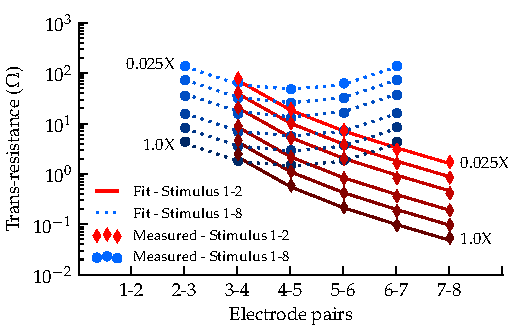
\includegraphics{graphics/pbs_transimpedance_IEEE}
    \end{center}
    \caption{Transresistance measurements (markers) used to generate the resistor mesh and the corresponding fit (lines). Red diamonds indicate results where a stimulus is placed across electrodes 1 and 2. Blue circles represent measurements where the stimulus is placed across electrodes 1 and 8. Each trace represents one of six concentrations of PBS, increasing in transresistance magnitude monotonically from 1.0X to 0.025X.}
    \label{fig:transresistance}
\end{figure}

\begin{table}
    \begin{center}
        \begin{tabular}{|r|l|}
            \hline
            $R_{eri}$ & 0.407 / $\sigma$ \\ \hline
            $R_{sri}$ & $R_{eri}$ $3/4$ \\ \hline
            $R_{li}$ & 3.71 / $\sigma$ \\ \hline
            Depth & 5 layers \\ \hline
            Padding & 3 layers \\ \hline
        \end{tabular}
    \end{center}
    \caption{Resistor mesh parameters. $\sigma$ measured in units of $S/cm$}
    \label{tab:RESparams}
\end{table}





\section{Displacement Parameters}

Displacement currents are responsible for capacitive behaviour at interfacial boundaries.
They are brought about by the redistribution of charge in response to applied fields, i.e. a charged electrode will attract or repel $Cl^{-}$ from its surface and reorientate polar molecules in the surrounding solution.\cite{Merrill05} This capacitive behaviour may also be a result of electrode polarisation in the form of reversible Faradaic reactions at the surface of the electrode.
Such reactions involving water and platinum, as identified in \cite{Horch2004,Mohtashami2011,Merrill05}, include:
\begin{eqnarray}
    Pt + H_{2}O &\Leftrightarrow& PtO + 2 H^{+} + 2 e^{-}\\
    PtO + H_{2}O &\Leftrightarrow& PtO_{2} + 2 H^{+} + 2e^{-}\\
    Pt + H^{+} & \Leftrightarrow & Pt-H\\
    Pt + H_{2}O + e^{-} &\Leftrightarrow& Pt-H+OH^{-}
\end{eqnarray}

This displacement mechanism is capable of transferring charge between electrical and biological systems without damaging electrodes or tissue.\cite{Horch2004}
This behaviour is modelled by way of a Constant Phase Element (CPE); also known as a fractional capacitor.
For simulation purposes this element is realised as an array of R-C branches.~\cite{ScottSingle2013,Morrison59,Elwakil10} where the value of each R-C pair is chosen to set the slope of impedance relative to frequency. The placement of R-C pairs within the CPE is determined by Morrison's parameters $m$ and $k$, where $k$ determines the spacing, or density, of R-C branches and $m$ determines the resulting slope.
We measure displacement currents by sweeping the frequency of a sinusoidal stimulus across electrodes 2 and 7 of the Octrode while measuring the voltage between electrodes 2 and 3 (numbering shown in Fig.~\ref{fig:octrode}).
This allows for the measurement of a single interface impedance in series with the resistance presented by the bulk solution.
\begin{figure}
    \begin{center}
        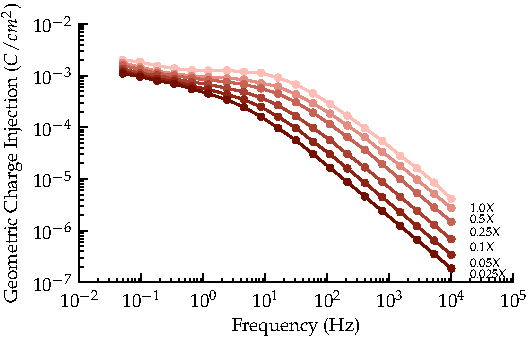
\includegraphics{graphics/chargeInjectionVsFrequency_magnitude}
    \end{center}
    \caption{Charge injected per phase during CPE measurement for each of the six concentrations of PBS. Calculated using a geometric surface area of 10\thinspace mm$^{2}$}
    \label{fig:chargeInjectionVsFrequency}
\end{figure}

The geometric current density during measurements peaked at 22.6\thinspace mA/cm$^{2}$ at 10000\thinspace kHz in 1.0X PBS and fell as low as 27.6\thinspace $\mu$A/cm$^{2}$ at 50\thinspace mHz in 0.025X PBS. Charge injection per phase is shown in figure~\ref{fig:chargeInjectionVsFrequency} for each solution.
The stimulus waveform was set at 300\thinspace mV (peak) at each measurement point. The measurement instruments used are the same as those used to measure the inter-electrode resistance.
Figure~\ref{fig:CPE_Magnitude} shows the magnitude of the measured response of each of the six PBS concentrations accompanied by simulation results. Figure~\ref{fig:CPE_Phase} shows the phase response for the same measurements, again with the simulated response at each concentration. The simulated responses are generated using the optimised parameter values presented in Table~\ref{tab:CPEparams}. Those values were chosen as they give the closest match to the measured data.

As shown in the interface model schematic (figure~\ref{fig:schematic}), the interface contains its own internal series resistance ($R_{S}$). The resistance seen in series with the CPE will therefore be the sum of both the resistance due to the bulk resistivity of the fluid and $R_{S}$, to which we will refer as $R_{S+bulk}$.
In figure~\ref{fig:CPE_Magnitude}, the slope and magnitude of the CPE are visible below 1\thinspace Hz whereas $R_{S+bulk}$  dominates above 1\thinspace kHz; it is clear that the two do not scale similarly.
As the impedance of the CPE and $R_{S+bulk}$ are separable with frequency, these measurements can be used to determine the CPE parameters and $R_{S}$.

Figure~\ref{fig:CPE_Scaling} shows measured data and the corresponding fits for both the CPE magnitude at 0.05\thinspace Hz and $R_{S+bulk}$. The model parameters $m$, $k$, $|Z|\thinspace @\thinspace 1Hz$, and $R_S$ are shown in table~\ref{tab:CPEparams}, with $|Z|\thinspace @\thinspace 1Hz$, and $R_S$ given as functions of concentration.
Here we express the CPE offset parameter as $|Z|\thinspace @ \thinspace 1Hz$, but the fits used $|Z|\thinspace @ \thinspace 0.05Hz$, as data points at this frequency are outside the transitional zone where the impedance of the CPE and that of $R_{S+bulk}$ overlap.

The data presented in Fig.~\ref{fig:CPE_Magnitude} show a large, linear, relative shift of $|Z|$ with salinity at higher frequencies, where the resistive component of the solution dominates.
Conversely, at lower frequencies where the $|Z|$ changes with frequency, the relative change is closer to logarithmic. This region is modeled by the CPE.
This suggests that the CPE does not chiefly rely on the added salt ions, but they do have some effect.
Instead, the constant-phase charge effect must arise from phenomena not associated with the salt ions.


\begin{figure}
    \begin{center}
        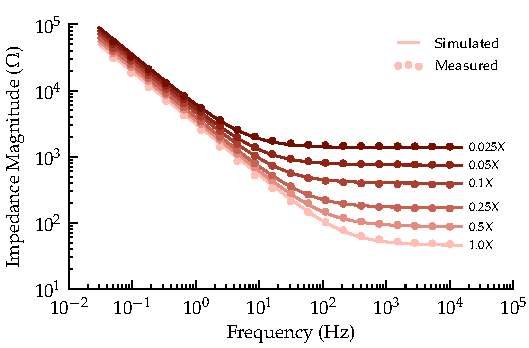
\includegraphics{graphics/displacement_impedanceVsFrequency_magnitude}
    \end{center}
    \caption{Magnitude of interfacial impedance between electrodes 2 and 7 against the frequency of a sine wave stimulus for six concentrations of PBS. The slope of the CPE is visible the left, whereas the resistance due to $R_{S+bulk}$ appears on the right. Traces represent simulated data while markers represent measured values.}
    \label{fig:CPE_Magnitude}
\end{figure}

\begin{figure}
    \begin{center}
        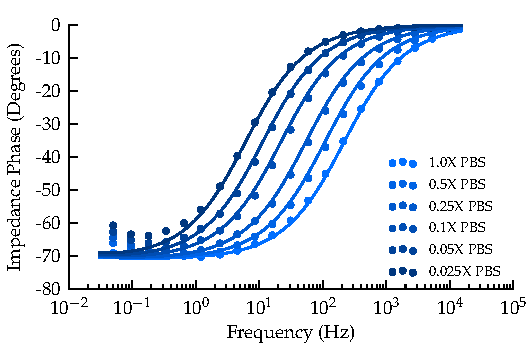
\includegraphics{graphics/displacement_impedanceVsFrequency_phase}
    \end{center}
    \caption{Phase data of interfacial impedance across electrodes 2 and 7 against frequency of a sine wave stimulus. Traces represent simulated data while markers represent measured values.}
    \label{fig:CPE_Phase}
\end{figure}

\begin{figure}
    \begin{center}
        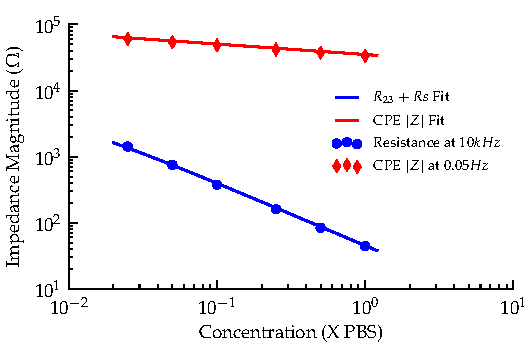
\includegraphics{graphics/scalingFactors_Displacement_IEEE}
    \end{center}
    \caption{Simulated and measured values of CPE parameters versus concentration of PBS. $|Z|$ is compared at 0.05\thinspace Hz as measured data is unaffected by $R_{S}$ at this frequency.}
    \label{fig:CPE_Scaling}
\end{figure}

\begin{table}
    \begin{center}
        \begin{tabular}{|r|l|}
            \hline
            $m$ & $1.34$ \\ \hline
            $k$ & $1.773$\\ \hline
            $|Z|\: @\: 1Hz$& $3284 \times concentration^{-0.158}$ \\ \hline
            $R_{S}$ & $13.38 \times concentration^{-0.8397} $\\ \hline
        \end{tabular}
    \end{center}
    \caption{Displacement parameter scaling}
    \label{tab:CPEparams}
\end{table}



\section{Faradaic Parameters}

With parameters fitted for the scaling of both the CPE and $R_{S}$ with PBS concentration, we turn to Faradaic conduction.

Our model uses two reverse connected diodes to represent Faradaic current conduction between electrode and electrolyte. Specifically we use the diodes to model irreversible Faradaic reactions. (Any reversible reactions, those producing reactants bound to the surface of the electrode, are encapsulated by the displacement branch (CPE) of the model.)
Possible irreversible Faradaic reactions for platinum electrodes in saline are:

\begin{align}
    Pt + 4Cl^{-} &\Rightarrow& [PtCl_{4}]^{2-} + 2 e^{-} \label{eqn:ptCl}\\
    2H_{2}O + 2 e^{-} &\Rightarrow& H_{2}\uparrow + 2OH^{-} \label{eqn:H20}\\
    2H_{2}O &\Rightarrow& O_{2}\uparrow + 4H^{+} + 4e^{-} \label{eqn:2H20}\\
    2Cl^{-} &\Rightarrow& Cl_{2}\uparrow + 2e^{-} \label{eqn:Cl} \\
    Cl^{-} + H_{2}O &\Rightarrow& ClO^{-} + 2H^{+} + 2e^{-} \label{eqn:ClH20}
\end{align}

{
    \color{blue}
    It should be noted that each of these reactions (\ref{eqn:ptCl}, \ref{eqn:H20}, \ref{eqn:2H20}, \ref{eqn:Cl} and \ref{eqn:ClH20}) have different reaction potentials. It is expected that the situation in-vivo will be much more complex.
}

The interface model uses the diodes to reproduce the exponential behaviour of Faradaic current conduction implied by the Butler-Volmer equation. We wish to measure this conduction by separating it from the displacement behaviour of the CPE. By using a DC measurement technique, as opposed to cyclic measurements, we are able to separate the effects in time.
Like a conventional capacitor, when the voltage across the CPE changes, it responds by absorbing or ejecting charge, causing a spike in current. The CPE will draw negligible current once it has settled and in the case of our model we assume the remaining current conduction to be the result of Faradaic processes.
In \cite{Greatbatch1969} it is shown that the stirring of an air-saturated solution of physiological saline reduces the settling time of platinum electrodes to stimulus transients; with both situations eventually settling to the same impedance.
The equation governing current conduction in a diode where the forward voltage across the diode, $V_{D}$, is small is
\begin{equation}
    I = i_{0}  e^{V_{D} / n V_{T}}
\end{equation}
where $V_{T}$ is the thermal voltage and is approximately 25\thinspace mV at a temperature of 300\thinspace K. We wish to find how the saturation current ($i_{0}$) and the ideality factor ($n$) scale as the solution salinity is varied.

Faradaic measurements were made using an Agilent E5270B Precision Measurement Mainframe producing a stepped DC voltage stimulus whilst continuously measuring the output current.

Measurements commenced with a 4.5 litre solution of 1.0X PBS which was progressively diluted in factors of two between each measurement. The solution was mixed continuously using a standard laboratory grade magnetic stirrer. The solution was in equilibrium with air prior to and during measurement and the electrodes remained submerged at all times.
A single measurement run involved stepping the voltage across the electrodes from 0.5\thinspace V to 1.2\thinspace V in increments of 0.05\thinspace V; this range was previously determined to capture the onset of Faradaic conduction.

In \cite{Cogan2008} it has been noted that results obtained using cyclic voltammetry are dependant on, among other factors, the measurement sweep rate. This indicates a lack of isolation between displacement and Faradaic mechanisms. Our measurements were repeated using wait-times of 4, 16, 32 and 64 seconds between voltage increments, allowing us to determine the effect of sweep rate. From these measurements and those of a separate investigation\footnote{We took measurements of the interface's response to voltage steps when left to settle for 10 000 seconds, of which the first 250\thinspace seconds are shown in figure~\ref{fig:CPE_currentVsTime}. Those measurements show a trend of decreasing current stabilisation time as the overpotential steps increase. Sixty four seconds after stepping from 0.64\thinspace V to 0.72\thinspace V, the current has stabilised to $95\%$ of its value at 10\,000 seconds. At overpotential steps for higher voltages, the settling time is further reduced. These measurements were made in still solution and we expect stirring will further reduce settling time.} we concluded that a wait-time of 64 seconds was sufficient.
\begin{figure}
    \begin{center}
        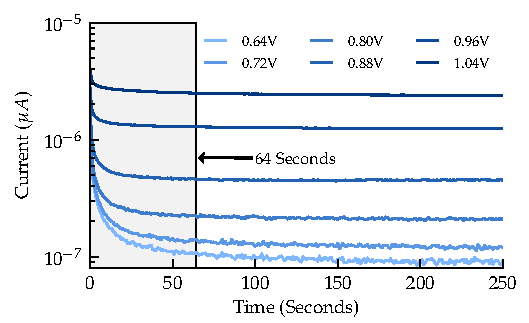
\includegraphics{graphics/CPE_currentVsTime}
    \end{center}
    \caption{Current versus time after a stepped voltage increment across a pair of interfaces. Time before 64 seconds is highlighted in grey. Measurements were taken with a wait time of 10,000 seconds between increments.}
    \label{fig:CPE_currentVsTime}
\end{figure}

In figure~\ref{fig:StepResponse_Faradaic}, electrical current measurements are plotted against time (solid lines). Each spike marks the point at which the voltage is incremented by 50\thinspace mV. Note that the amount of charge absorbed by the CPE increases with concentration of PBS, but the current for each concentration converges to approximately the same value. Dotted lines have been added that link the electrical current measurements taken 10 seconds after each increment for 0.125X PBS (lower trace) and 1.0X PBS (upper trace). These dotted traces show results typical of cyclic methods, where the electrode overpotential is never constant. This illustrates the benefit of using DC measurements when measuring Faradaic currents.

Figure~\ref{fig:faradaic_logCurrentVsVoltage} shows the settled currents plotted on a log scale, versus the voltage applied across the electrodes. This uses the same data as the previous figure but has been processed so that each point represents the average of the final 24 current measurements at each step. Below 0.9\thinspace V it appears that the concentration of the solution had no identifiable effect on Faradaic conduction as there is overlap between each trace and the mean values are not monotonic with concentration in this region.  Between 0.9\thinspace V and 1.05\thinspace V a transition occurs which results in current conduction becoming dependent on solution concentration.
Above 1.05\thinspace V the traces diverge showing clear dependence upon concentration.
The point at which this transition occurs is determined by the concentration of saline, with lower concentrations transitioning earlier. A concentration of 0.0625X PBS causes a transition at around 0.95\thinspace V whereas electrodes in the 1.0X PBS solution transition somewhere between 1.0\thinspace and 1.05\thinspace V. The effect of transition can be seen in the green trace at 1.0\thinspace V where the error bar is wide due to the current shift being captured in the measurement at that voltage. Part of a transition with respect to time is visible in figure~\ref{fig:StepResponse_Faradaic} where the red trace drops uncharacteristically after the increment at around 600 seconds.

\begin{figure}
    \begin{center}
        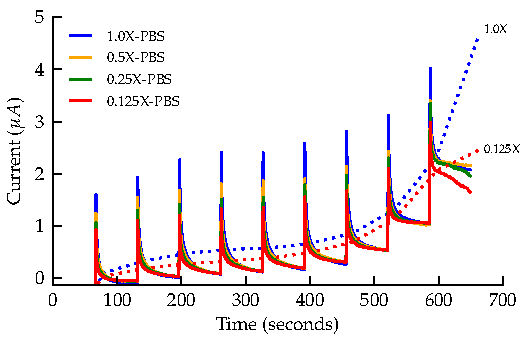
\includegraphics{graphics/currentTimeFaradaicCPE_Stacked_IEEE}
    \end{center}
    \caption{Current conduction with 0.05\thinspace V stepped voltage increments from 0.5\thinspace V to 0.9V. Each voltage is held for 64 seconds before being further incremented. Dotted lines connect current measurements occurring 10 seconds after an increment.}
    \label{fig:StepResponse_Faradaic}
\end{figure}


\begin{figure}
    \begin{center}
        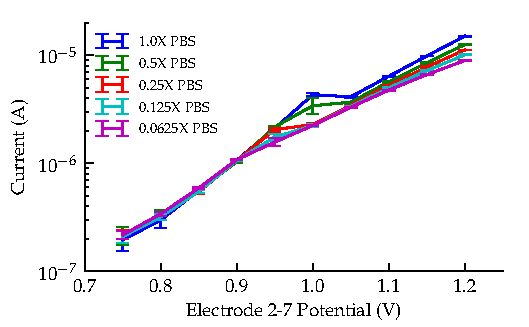
\includegraphics{graphics/currentVoltage_logY_IEEE}
    \end{center}
    \caption{Faradaic conduction as a function of voltage applied across electrodes 2 and 7. Samples shown were taken between 40 and 64 seconds after each voltage increment. Error bars indicate spread in measurement results, where 95\% of samples lie within the bars.}
    \label{fig:faradaic_logCurrentVsVoltage}
\end{figure}

\begin{figure}
    \begin{center}
        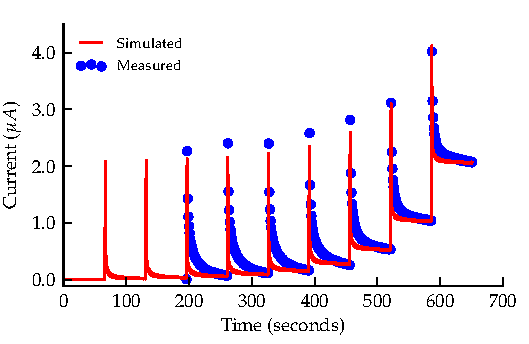
\includegraphics{graphics/faradaic_currentVsTimeIEEE}
    \end{center}
    \caption{Current versus time for 1.0X PBS overlaid with simulated results of the interface model's response to increasing voltage steps. The model used for simulation includes the CPE, diodes and $R_{S}$.}
    \label{fig:faradaic_currentVsTime}
\end{figure}

\begin{figure}
    \begin{center}
        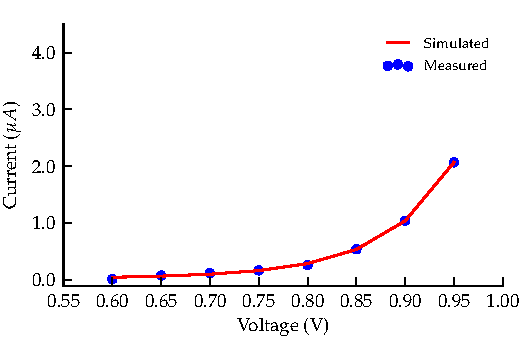
\includegraphics{graphics/faradaic_currentVsVoltageIEEE}
    \end{center}
    \caption{Simulated response of the interface model compared to measurement from the electrodes with a stepped voltage overpotential. Measurement points show current values taken at the $64^{th}$ second after each voltage increment.}
    \label{fig:faradaic_currentVsVoltage}
\end{figure}

\begin{table}
    \begin{center}
        \begin{tabular}{|r|l|}
            \hline
            $i0$ & 2.757e-12\\ \hline
            $n$ & 1.36\\ \hline
        \end{tabular}
    \end{center}
    \caption{Faradaic parameters}
    \label{tab:FaradaicParams}
\end{table}

%Parameter values for $i_{0}$ and $n$ are presented in table~\ref{tab:FaradaicParams}. These parameters were found by fitting the diode equation to the results shown in figure~\ref{fig:faradaic_currentVsVoltage}.

We attribute the change in behaviour between 0.9\thinspace V and 1.05\thinspace V to a transition to diffusion-controlled conduction.
We hypothesise that the charging of the CPE draws available ions to the electrode, creating a layer of high ionic concentration at the surface irrespective of that of the solution bulk. It is this layer that is subsequently consumed by the Faradaic reactions at a {\color{blue} rate that increases exponentially with} electrode overpotential.  The effect of bulk solution concentration while this layer has formed is negligible until the point at which the layer is consumed faster than it can be replenished. At this stage, and with increasing overpotential, the Faradaic conduction is governed by diffusion of ions from the bulk into the layer, the rate of which increases with the ion concentration in the bulk. We believe this explains the divergence of conduction with concentration between 0.9\thinspace V and 1.05\thinspace V and why there is no observable dependence on bulk ion concentration beforehand.
For the purposes of our model, we are content with placing a limit of 0.9\thinspace V across the pair of interfaces and using the assumption that Faradaic conduction does not change with concentration.


    Figure~\ref{fig:faradaic_currentVsTime} shows a subset of the data used in Fig.~\ref{fig:StepResponse_Faradaic} (the 1.0X PBS trace) to show the fit between simulated and measured data in the time domain. Here the simulation contains fitted diode parameters, shown in table~\ref{tab:FaradaicParams}, which give rise to the exponentially increasing steady state current.
It is apparent from this trace that the temporal response of the CPE does not match the transient decay curves seen in the Faradaic measurements, something the CPE should predict. These transient decay curves appear to have a time-constant\footnote{We use the term ``time-constant'' although a CPE does not have a simple exponential time-domain response.} that decreases with each subsequent measurement. This variable time-constant phenomena is especially clear when looking back at figure~\ref{fig:CPE_currentVsTime}. Although the Faradaic response transients appear to approach the time-constant predicted by the CPE, there is still behaviour not completely described by the CPE.

The match between fitted diode parameters ($n$ and $i_{0}$) and the measurement data 64 seconds after each voltage increment has been plotted in figure~\ref{fig:faradaic_currentVsVoltage}.

In future we hope to extend this model into a diffusion controlled conduction scenario and extend the CPE element to better reproduce the time domain response.





\section{In-vivo measurements of sheep}

\begin{figure}
    \begin{center}
        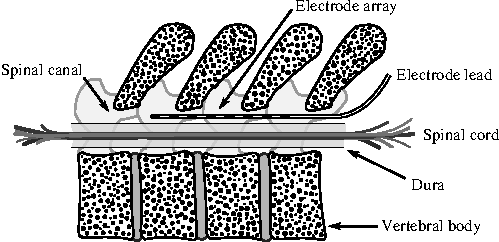
\includegraphics{graphics/sheepSpine}
    \end{center}
    \caption{Cross section of a sheep spine showing the position of the electrode array relative to the dura. Spotted regions represent cross sectioned vertebrae.}
    \label{fig:sheepSpine}
\end{figure}
Cogan states the main differences between in-vivo and in-vitro responses come down to temperature, the presence of organic species, tortuous diffusion path for charge carriers, physiological responses of the host to a foreign body, and uncertain concentrations of electrolytes and buffers near the electrode surface.\cite{Cogan2008}
Nevertheless, electrical engineers use baths of saline as a substitute for in-vivo testing (a ``phantom'') due to its convienience.
We now test the claim that 0.1X PBS is a reasonable representation of the spine of a living sheep.

The displacement measurements were repeated inside the spinal canal of a live sheep, just outside the dura as shown in figure~\ref{fig:sheepSpine}. The sheep were prepared and anaesthetised using the procedures described in \cite{Parker2013} under the Animal Care and Ethics Committee approval of the Royal North Shore Hospital, Sydney. The study complied with the Australian Code of Practice for the Care and Use of Animals for Scientific Purposes.
Four measurements taken at regular intervals over a period of 30 minutes are presented in figures~\ref{fig:displacement_sheepCPEMagnitude} and~\ref{fig:displacement_sheepCPEPhase} on top of the array of traces for saline taken from figures~\ref{fig:CPE_Magnitude} and~\ref{fig:CPE_Phase}.
Although it is clear that there are complications in vivo, a 0.25X PBS saline offers a good approximation to the resistive part of the trace.
The reactive part would be better modelled by a solution of less than 0.025X concentration.

\begin{figure}
    \begin{center}
        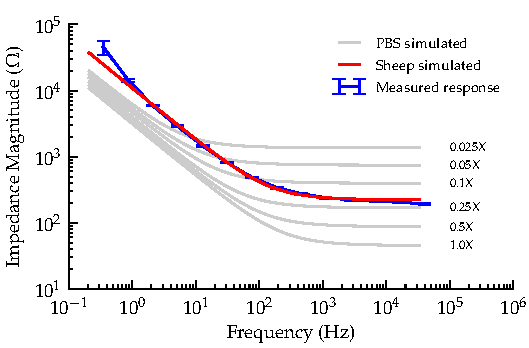
\includegraphics{graphics/displacement-withSheep_impedanceVsFrequency_magnitude}
    \end{center}
    \caption{Comparison between the magnitude of CPE in live sheep (blue error bars) against each of the PBS traces from figure~\ref{fig:CPE_Magnitude} (grey lines) and a simulated fit to the sheep data (red trace).}
    \label{fig:displacement_sheepCPEMagnitude}
\end{figure}

\begin{figure}
    \begin{center}
        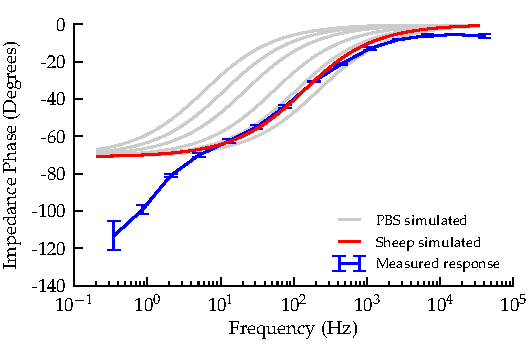
\includegraphics{graphics/displacement-withSheep_impedanceVsFrequency_phase}
    \end{center}
    \caption{Comparison between the phase response of the CPE in live sheep (blue error bars) against each of the PBS traces taken from figure~\ref{fig:CPE_Phase} (grey lines) and a simulated fit to the sheep data (red trace).}
    \label{fig:displacement_sheepCPEPhase}
\end{figure}

\section{Conclusion}

We have used the parameters of a compact electrical model of an implantable electrode as a way of objectively comparing scenarios.
We have measured how changing the concentration of PBS affects the parameters of this model.
We have drawn direct relationships with concentration sufficient to predict interface characteristics at arbitrary dilutions of PBS.
We found that the magnitude of the CPE element moves much more slowly with concentration whereas the resistance moved almost linearly.
Using DC measurements we conclude that the salinity of the bulk does not affect Faradaic conduction until a threshold voltage is reached. We hypothesise that this is because the double-layer sets the effective concentration of ions in a localised volume surrounding each electrode. In-vivo measurements of platinum electrodes in sheep spine showed that no single concentration of PBS matches both the CPE and the resistive characteristics at once. Nevertheless, 0.1X PBS is a good compromise.

\section*{Acknowledgment}
The authors wish to acknowledge the The University of Waikato for financial support and Saluda Medical for the use of facilities and equipment.

\begin{thebibliography}{99}


\bibitem{Cogan2008}
    Stuart~F.~Cogan,
    ``Neural Stimulation and Recording Electrodes'',
    Annu. Rev. Biomed. Eng. 2008. pp275--309.

\bibitem{Troy2006}
    John~B.~Troy, Donald~R.~Cantrell, Allen~Taflove and Rodney~S.~Ruoff
    ``Modeling the electrode-electrolyte interface for recording and stimulating electrodes'',
    {\em Proceedings of the 28th IEEE EMBS Annual International Conference}
    New York City, USA, Aug. 30, 2006, pp879--881.

\bibitem{Franks2005}
W.~Franks, Iwan~Schenker, Patrik~Schmutz, and Andreas Hierlemann,
``Impedance Characterization and Modeling of Electrodes for Biomedical Applications'',
\emph{IEEE Transactions on Biomedical Engineering},
vol.~52 no.~7, July 2005, pp1295--1302.

\bibitem{Mohtashami2011}
    Saba~Mohtashami,
    ``Electrochemical Properties of Flexible Electrodes for Implanted Neuromuscular Excitation Applications'',
    Open Acess Dissertations and Theses (2011), Paper 6152

\bibitem{Horch2004}
    K.~W.~Horsch and G.~S.~Gurpreet,
    ``Neuroprosthetics: theory and practice'',
    World Scientific, 2004.

\bibitem{ScottSingle2013}
Jonathan Scott and Peter Single,
``Compact Nonlinear Model of an Implantable Electrode Array for Spinal Cord Stimulation (SCS)'',
to be published in
{\em IEEE Transactions on Biomedical Circuits and Systems},
DOI: 10.1109/TBCAS.2013.2270179, 2013.

\bibitem{Kane13}
Sheryl~R.~Kane, Stuart~F.~Cogan, Julia~Ehrlich, Timothy~D.~Plante, Douglas~B.~McCreery and Philip~R.~Troyk,
``Electrical Performance of Penetrating Microelectrodes Chronically Implanted in Cat Cortex``,
{\em IEEE Transactions on Biomedical Engineering},
vol.~60 no.~8, August 2013, pp2153--2160.

\bibitem{Merrill05}
Daniel~R.~Merrill, Maron Bikson and John~G.~R.\ Jefferys,
``Electrical stimulation of excitable tissue: design of efficacious and safe protocols'',
Journal of Neuroscience Methods 141 (2005), pp171--198.

\bibitem{StJudeOctrode}
St.~Jude Medical, Octrode Percutaneous Lead for Neuromodulation,
\url{http://www.sjmneuropro.com/Products/US/Percutaneous-Leads.aspx},
retrieved December 2012.

\bibitem{Greatbatch1969}
W.~Greatbatch, B.~Piersma, F.~D.~Shannon, and S.W.~Calhoon, S. W.
``Polarization phenomena relating to physiological electrodes'',
Annals of the New York Academy of Sciences,
167(2), 1969 pp722-744.

\bibitem{Morrison59}
Ralph Morrison,
``RC Constant-Argument Driving-Point Admittances'',
{\em IRE Transactions on Circuit Theory},
September 1959, pp310--317.

\bibitem{Elwakil10}
Ahmed~S.~Elwakil,
``Franctional-Order Circuits and Systems: An Emerging Interdisciplinary Research Area''
IEEE Circuits and Systems Magazine, Fourth quarter, 2010, pp40--50.

\bibitem{Parker2013}
Parker J.L., Karantonis D.M., Single P.S., Obradovic M., Laird J., Gorman R.B., Ladd L.A., Cousins M.J.,
``Electrically Evoked Compound Action Potentials Recorded From the Sheep Spinal Cord'',
Neuromodulation 2013; 16: 295--303.

%%%%%%%%%%%%%%%%%%%%%%%%%%%%%%%%%%%%%%%%%%%%
% Check that these are in the right order!!!
%%%%%%%%%%%%%%%%%%%%%%%%%%%%%%%%%%%%%%%%%%%%

\bibitem{Weiland2000}
Weiland~James~D. and Anderson~David~J.,
``Chronic Neural Stimulation with Thin-Film, Iridium Oxide Electrodes'',
{\em IEEE Transactions on Biomedical Circuits and Systems},
vol.~47 no.~7, July 2000, pp911--918




\end{thebibliography}


\begin{IEEEbiography}[{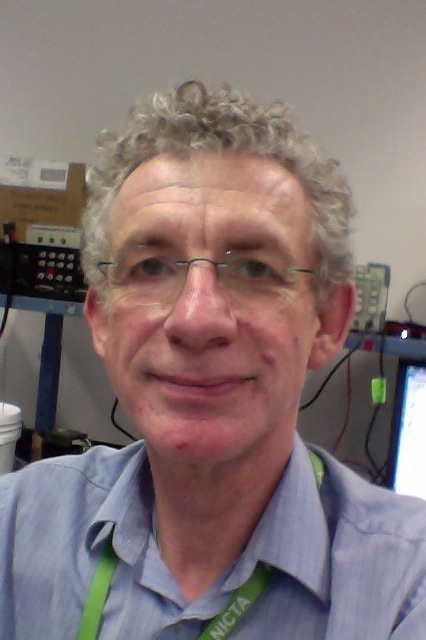
\includegraphics[width=1in,height=1.25in,clip,keepaspectratio]{graphics/JBSatNICTA.jpg}}]{Jonathan Scott}
(M'80--SM'99) is the Foundation Professor in
Electronic Engineering at the University of Waikato in Hamilton, New
Zealand.  From 1998 to 2006 he was with the Hewlett-Packard,
now Agilent Technologies, Microwave Technology Center in Santa Rosa,
where he was responsible for advanced measurement systems.  In 1997 and
1998 he was Chief Engineer at RF Technology in Sydney.  He was with The
University of Sydney in the Department of Electrical Engineering prior
to 1997.  He is a Professorial Fellow of Macquarie
University.  Professor Scott has authored over 100 refereed
publications and holds a number of patents.
\end{IEEEbiography}


\begin{IEEEbiography}[{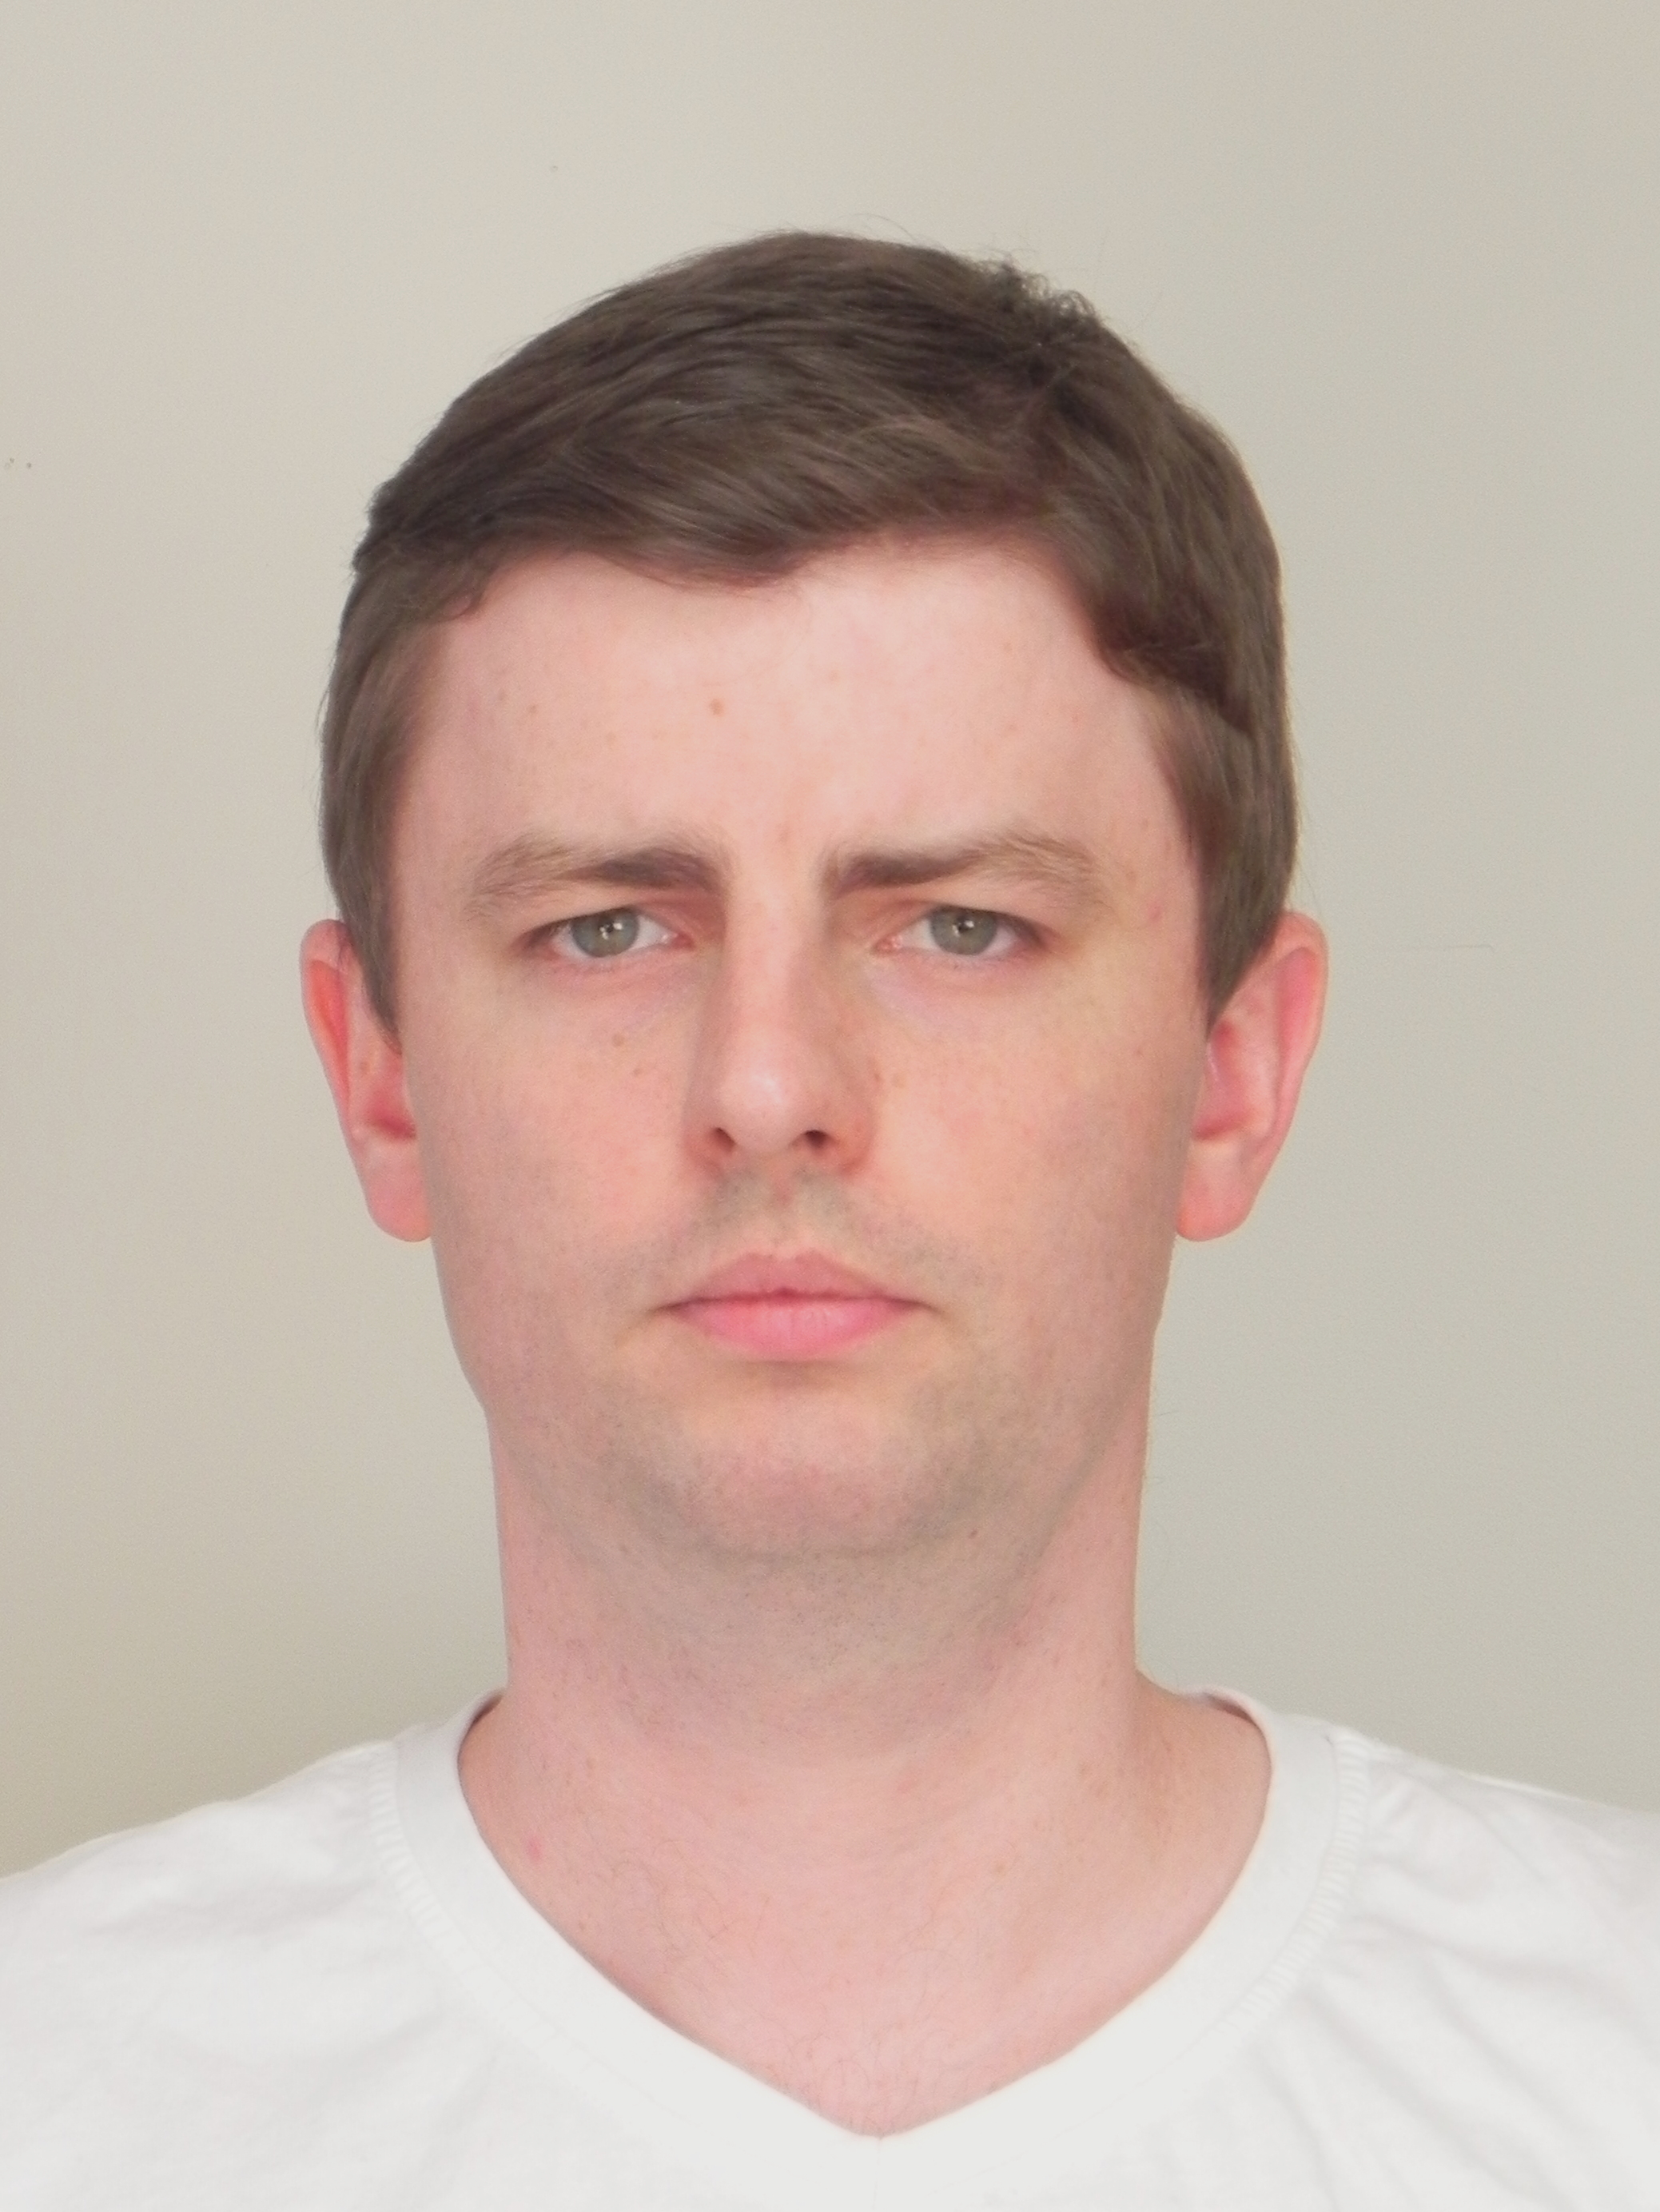
\includegraphics[width=1in,height=1.25in,clip,keepaspectratio]{graphics/MarkJones-Aug13.jpg}}]{Mark Jones}
received the B.Sc. degree in Physics in 2008 and the M.E. degree in Microwave Electronics in 2009 from The University of Waikato, Hamilton, New Zealand.
He is working towards a Ph.D. in Electrical Engineering, also at The University of Waikato.
\end{IEEEbiography}

\section*{Reviewers' Comments to the Authors:}

\subsection*{Reviewer: 1}

Comments to the Author

{
    \color{OliveGreen}
    My comments have been sufficiently addressed.
}

{
    \color{blue}
    Thank you.
}


\subsection*{Reviewer: 2}

Comments to the Author

{
    \color{OliveGreen}
    Required modification done and manuscript now significantly improved.
}

{
    \color{blue}
    Thank you.
}

\subsection*{Reviewer: 3}

Comments to the Author

{\color{OliveGreen}
    I am sorry to say that the revised version of the paper is still quite unsatisfactory. You have added electrochemical reactions (5)-(9) but do not acknowledge that these all have different reaction potentials, will have different charge transfer coefficients ( alpha in the Butler Volmer equation http://en.wikipedia.org/wiki/Butler\%E2\%80\%93Volmer\_equation), and will by limited by mass transfer to different extents. Therefore the use of diodes in the model is not obviously appropriate.

    {\color{blue}
        The diodes are there to model the change in current attributed to the first biologically damaging reaction that occurs at the electrode/electrolyte interface. Whatever reaction occurs first in the relevant electrolyte is the reaction that diode aims to mimic. We observe that the current increases near exponentially around this point so we use a diode to mimic that. We expect this reaction may not be the same in-vivo as it is in-vivo but the properties of a diode can be altered to match where this occurs.

        If there are secondary reactions occurring at higher potentials then we could add a second pair of diodes with the properties of that specific reaction. The problem here is that we would then need to include memristors (as used in ScottSingle2013) to account for reactant depletion. We don't account for reactant depletion for the same reason we don't account for reactions other than the very first Faradaic reaction to occur. The reason is that we never want biologically damaging reactions to occur due to an implant, so if they happen then something has gone wrong.

        Think of our attempt to model Faradaic reactions as a ``you've pushed this too far'' indicator for an electrical engineer.

        I think you're essentially right with you're argument, we're not up-front about this and we probably portray more capability in the Faradaic modelling aspect than we are able or aim to achieve.
    }

    My interpretation of your data in Fig 10 is this. Above 1.05V, the electrolysis reactions (6) and (7) are occurring and the current will partly depend on the conductivity (therefore concentration) of the electrolyte. Below about 1.05V, the direct current may indeed be due to oxygen reduction at the cathode and oxygen evolution at the anode, which you cite (page 1, col 2, line 53) from ref 10 (c.f. Clark Oxygen Electrode). In that case, dissolved oxygen will have to diffuse to the cathode because it is not charged, so this will be diffusion-limited, which explains why the current is independent of concentration. Maybe you disagree with me but it is unsatisfactory that this is speculative and no doubt you will say that you did not want to get involved in electrochemistry, you just wanted to construct a model.

    {
        \color{blue}
        Correct, we do not wish to determine exactly what is happening at the electrode surface - we want to create a flexible model that can be used to simulate impedance.

    }


    Even as a model, however, your case is not very convincing.

    1. You state in the Introduction that you aim for a model suitable for stimulation yet there are no results comparing the model with experiment when the electrodes are used in this way. All the results are with sinusoidal excitation (which are of low amplitude at high frequencies), or DC with steps.

    {
        \color{blue}
        This is a good point. ScottSingle2013 compare the model prediction to stimulus waveforms. Our aim is to see what changes in that model as the concentration of PBS is varied and to compare those measurements to in-vivo measurements using a live sheep. Were doing this because 0.1X PBS is commonly used as a phantom for real spine. There hasn't been an objective way of determining how accurate that assumption was until we used this model to make that comparison.
    }

    2. Your model of the interface (Fig 2) has a series resistor Rs. I do not see why you need this and how you can measure it: how do you separate it from the volume resistance (``Resistive Network'')? (You mention this on p3 col 1, line 55 without casting any light.)

    {
        \color{Blue}
        We need this because it represents the resistance of the interface itself, separate from that of the fluid.
        We measure the impedance magnitude of the displacement currents at high frequency (flattened part of Fig. 5). For each concentration the impedance magnitude at 10kHz is higher than is predicted by the transimpedance measurements made in Fig. 3. The transimpedance measurments do not measure impedance across an interface that is passing current and therefore any voltage drop across an interface due to $R_{S}$ would vanish. The displacement measurements take the voltage across interfaces that are passing stimulus currents. These measurements see the potential drop across the interface due to the current flow via Ohms law.

        The transimpedance measurements give us an interelectrode resistance. The displacement measurements at high frequency give us an interelectrode impedance plus an interface impedance. Subtracting one from the other gives us a value of resistance that only appears as we pass current through an interface, which we include as $R_{S}$.
    }

    3. The maximum charge limit for Pt was given by Brummer \& Turner (IEEE Trans BME, 24, 436-9, 1977) as 320 microcoulombs per cm\^2, and later authors revised this downward. If you really applied the charge density that you show in Fig 4, you exceeded this limit at frequencies below ~50Hz and I would expect that your electrodes would have been gassing. In that case it is surprising that the impedance curves in Figs 5 \& 6 do not show a deviation from pure CPE behaviour. This is an important anomaly.

    4. The time constants seen in Figs 8, 9 \& 11 are interesting. Fig 11 shows that the model does not fit well because its time constant is too short. But is this surprising? Your impedance spectra go down to 0.05Hz (Figs 4-6) and I suppose that you chose RC pairs for your CPE model that go down to that frequency. But that is only to a time constant of ~3s (1/2*pi*f) which is much less that the 250s in Fig 8. It would be interesting to know whether, if you extended the spectrum far enough down, the time constants from step changes to the RC network that approximates the CPE would be similar to those seen in Fig 8.

    {
        \color{blue}
        The RC pairs are generated via a Python script for a given frequency range.
    }

    5. p 6, col 1, line 11. ``rate dependent on the log'' should be ``rate varies exponentially''. i.e. Tafel equation.
    
    {
        \color{blue}
        Correct, change made.
    }

    6. Figs 14 \& 15 are intriguing. For reason given in 3 above, I discount the results below 50Hz, yet it does look as if the slope of the CPE is the same in vivo but with an offset that would correspond to a very weak solution of PBS. As far as I know, there is no satisfactory explanation yet for the CPE so perhaps this is a significant clue.
}

\subsection*{Reviewer: 4}

Comments to the Author

{
    \color{OliveGreen}
    In this manuscript, the authors studied the impedance of a commercial electrode array as a function of concentration of phosphate buffered saline (PBS), both through simulation and empirical measurements, and compared those results to the impedance measured when the electrode array was implanted into a sheep's spinal cavity. From this comparison, they concluded that the current practice of testing spinal cord stimulator in 0.1x of physiologically normal saline is adequate but suggest that no single concentration of PBS captures the frequency dependence of the in vivo measured impedance. Although not a very compelling conclusion, this manuscript does provide value to the field as a single source for creation of a compact, SPICE model of an electrode. Hence, my review is cast in the light of using this paper as a guide in developing a model of a different electrode.

    1. As much of the paper involves development of the model, I recommend that the authors add some reference to modeling in the abstract.

    2. Sections 2, 3, and 4 detail the measurement and simulation of measurements of parameters associated with the bulk solution, CPE and Rs, and the diodes of the model in Figure 2. I recommend that the authors expand the introduction to explain this organization to help the reader's understanding. Additionally, I propose that the authors expand the section headings to include this information.

    3. The parameters provided in Table II include reference to an unexplained term sigma (σ). I presume this is the conductivity of saline (correct symbol and units for conductivity). For completeness, I recommend the authors explain this term, provide the numeric value (or values) that they used, provide how they adjusted this with concentration, and reference the source of their numeric data.

    4. From the parameters provided in Table II, I can guess how many elements are in the SPICE model arising from these parameters but it would be much more valuable to the reader to have a clear statement of the true size of the associated SPICE model. I recommend the authors provide a clear statement at the end of this section of how many resistors are in their SPICE model as a result of this parameterization.

    5. In Section 3, the authors state that the CPE is modeled as an array of R-C branches but at no time do they state the actual number of branches used in their model. I recommend the authors provide a clear statement at the end of this section of how many capacitors and resistors are in their SPICE model because of this parameterization.

    6. The parameters provided in Table II include reference to `concentration'. As different readers will have different interpretations (mass concentration=0.9\%, molar concentration = 0.154M), I recommend the authors clearly explain the meaning of this term.

    7. Given the authors details 3 different parts of their model in Sections 2, 3, and 4, I found it surprising that they only chose to characterize CPE in their in vivo experiment. In other words, if the complete model is important to performing simulation studies of a stimulation system, why did they not do such in their in vivo model and how valuable is their conclusion regarding the applicability of using 0.1xPBS as an in vitro of an animal. At minimum, I recommend the authors explain why they only characterized CPE in vivo.

    8. In the conclusions, I recommend the authors provide details on the overall size of their SPICE model. Knowing this information, a reader can compare the compactness of the complete model to that of using a finite element model.

    9. In their conclusions, I recommend the authors restate any limitations in their model that they mentioned earlier in the text (e.g., 0.9v limitation) and provide an honest discussion regarding the limits of their model.
}



\end{document}
